%%%%%%%%%%%%%%%%%%%%%%%%%%%%%%%%%%%%%%%%%
% University/School Laboratory Report
% LaTeX Template
% Version 3.1 (25/3/14)
%
% This template has been downloaded from:
% http://www.LaTeXTemplates.com
%
% Original author:
% Linux and Unix Users Group at Virginia Tech Wiki
% (https://vtluug.org/wiki/Example_LaTeX_chem_lab_report)
%
% License:
% CC BY-NC-SA 3.0 (http://creativecommons.org/licenses/by-nc-sa/3.0/)
%
%%%%%%%%%%%%%%%%%%%%%%%%%%%%%%%%%%%%%%%%%

%----------------------------------------------------------------------------------------
%	PACKAGES AND DOCUMENT CONFIGURATIONS
%----------------------------------------------------------------------------------------

\documentclass{article}

\usepackage{graphicx} % Required for the inclusion of images
\usepackage{natbib} % Required to change bibliography style to APA
\usepackage{amsmath} % Required for some math elements
\usepackage{mathtools}
\usepackage[export]{adjustbox}
\usepackage{subcaption}
\usepackage{float}
\usepackage{listings}
\usepackage{minted}

\DeclarePairedDelimiter{\abs}{\lvert}{\rvert}
\setlength\parindent{0pt} % Removes all indentation from paragraphs

\renewcommand{\labelenumi}{\alph{enumi}.} % Make numbering in the enumerate environment by letter rather than number (e.g. section 6)

%\usepackage{times} % Uncomment to use the Times New Roman font

%----------------------------------------------------------------------------------------
%	DOCUMENT INFORMATION
%----------------------------------------------------------------------------------------

\title{ECE 637 Digital Image Processing Laboratory: \\ Image 
Restoration} % Title

\author{Yang \textsc{Wang}} % Author name

\date{\today} % Date for the report

\begin{document}

\maketitle % Insert the title, author and date

%----------------------------------------------------------------------------------------
%	SECTION 1
%----------------------------------------------------------------------------------------
\section{Minimum Mean Square Error (MMSE) Linear Filters}

\subsection{Plot Original Four Images}
	\begin{figure}[h]
		\begin{subfigure}{0.5\textwidth}
			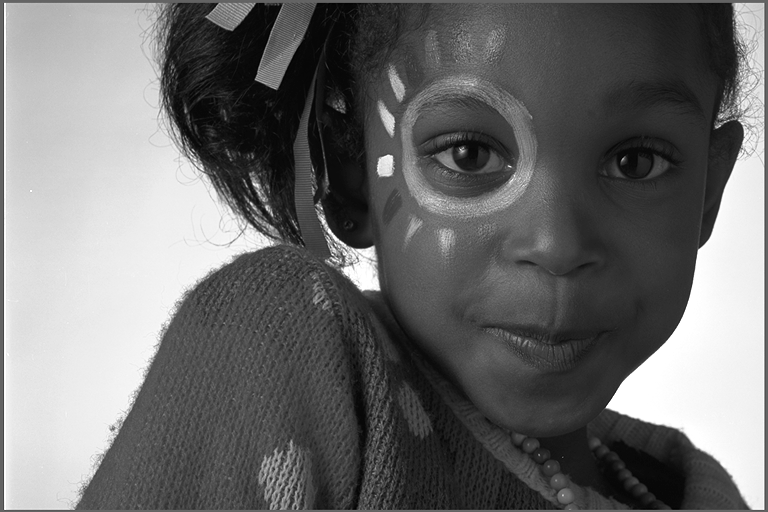
\includegraphics[width=1.0\textwidth]{img14g.png}
			\caption{img14g.tif}
		\end{subfigure}
		\begin{subfigure}{0.5\textwidth}
			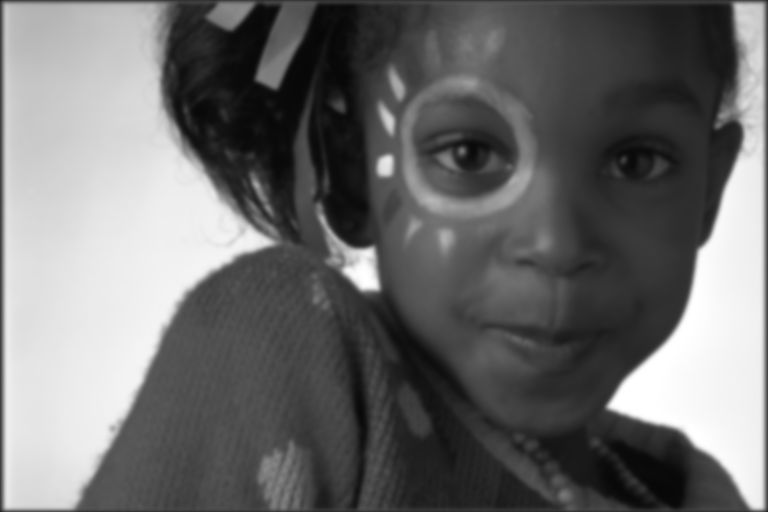
\includegraphics[width=1.0\textwidth]{img14bl.png}
			\caption{img14bl.tif}
		\end{subfigure}
		\begin{subfigure}{0.5\textwidth}
			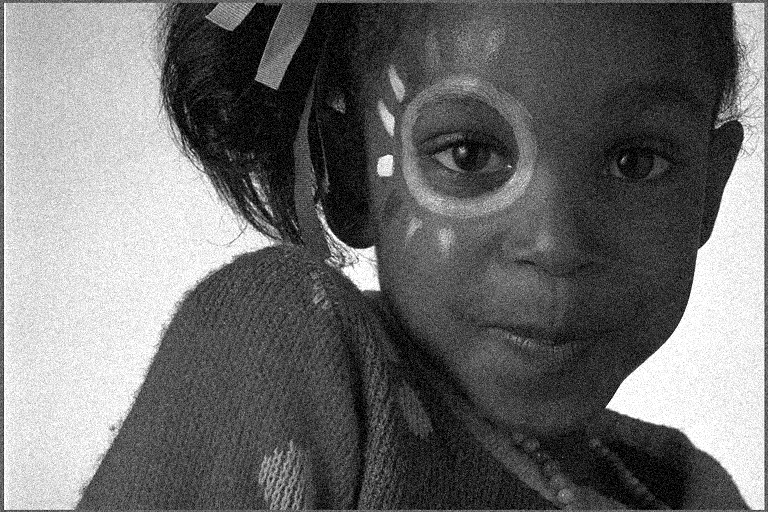
\includegraphics[width=1.0\textwidth]{img14gn.png}
			\caption{img14gn.tif}
		\end{subfigure}
		\begin{subfigure}{0.5\textwidth}
			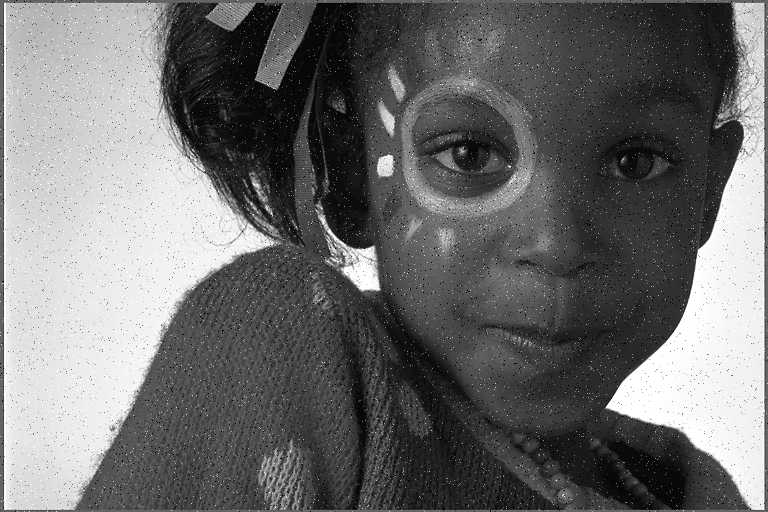
\includegraphics[width=1.0\textwidth]{img14sp.png}
			\caption{img14sp.tif}
		\end{subfigure}
		\caption{Orignal Fabulous Four Images}
	\end{figure}

\subsection{Plot the Blurred Image, and Two Noisy After Optimal Filtering}
	\begin{figure}[h]
		\begin{subfigure}{0.5\textwidth}
			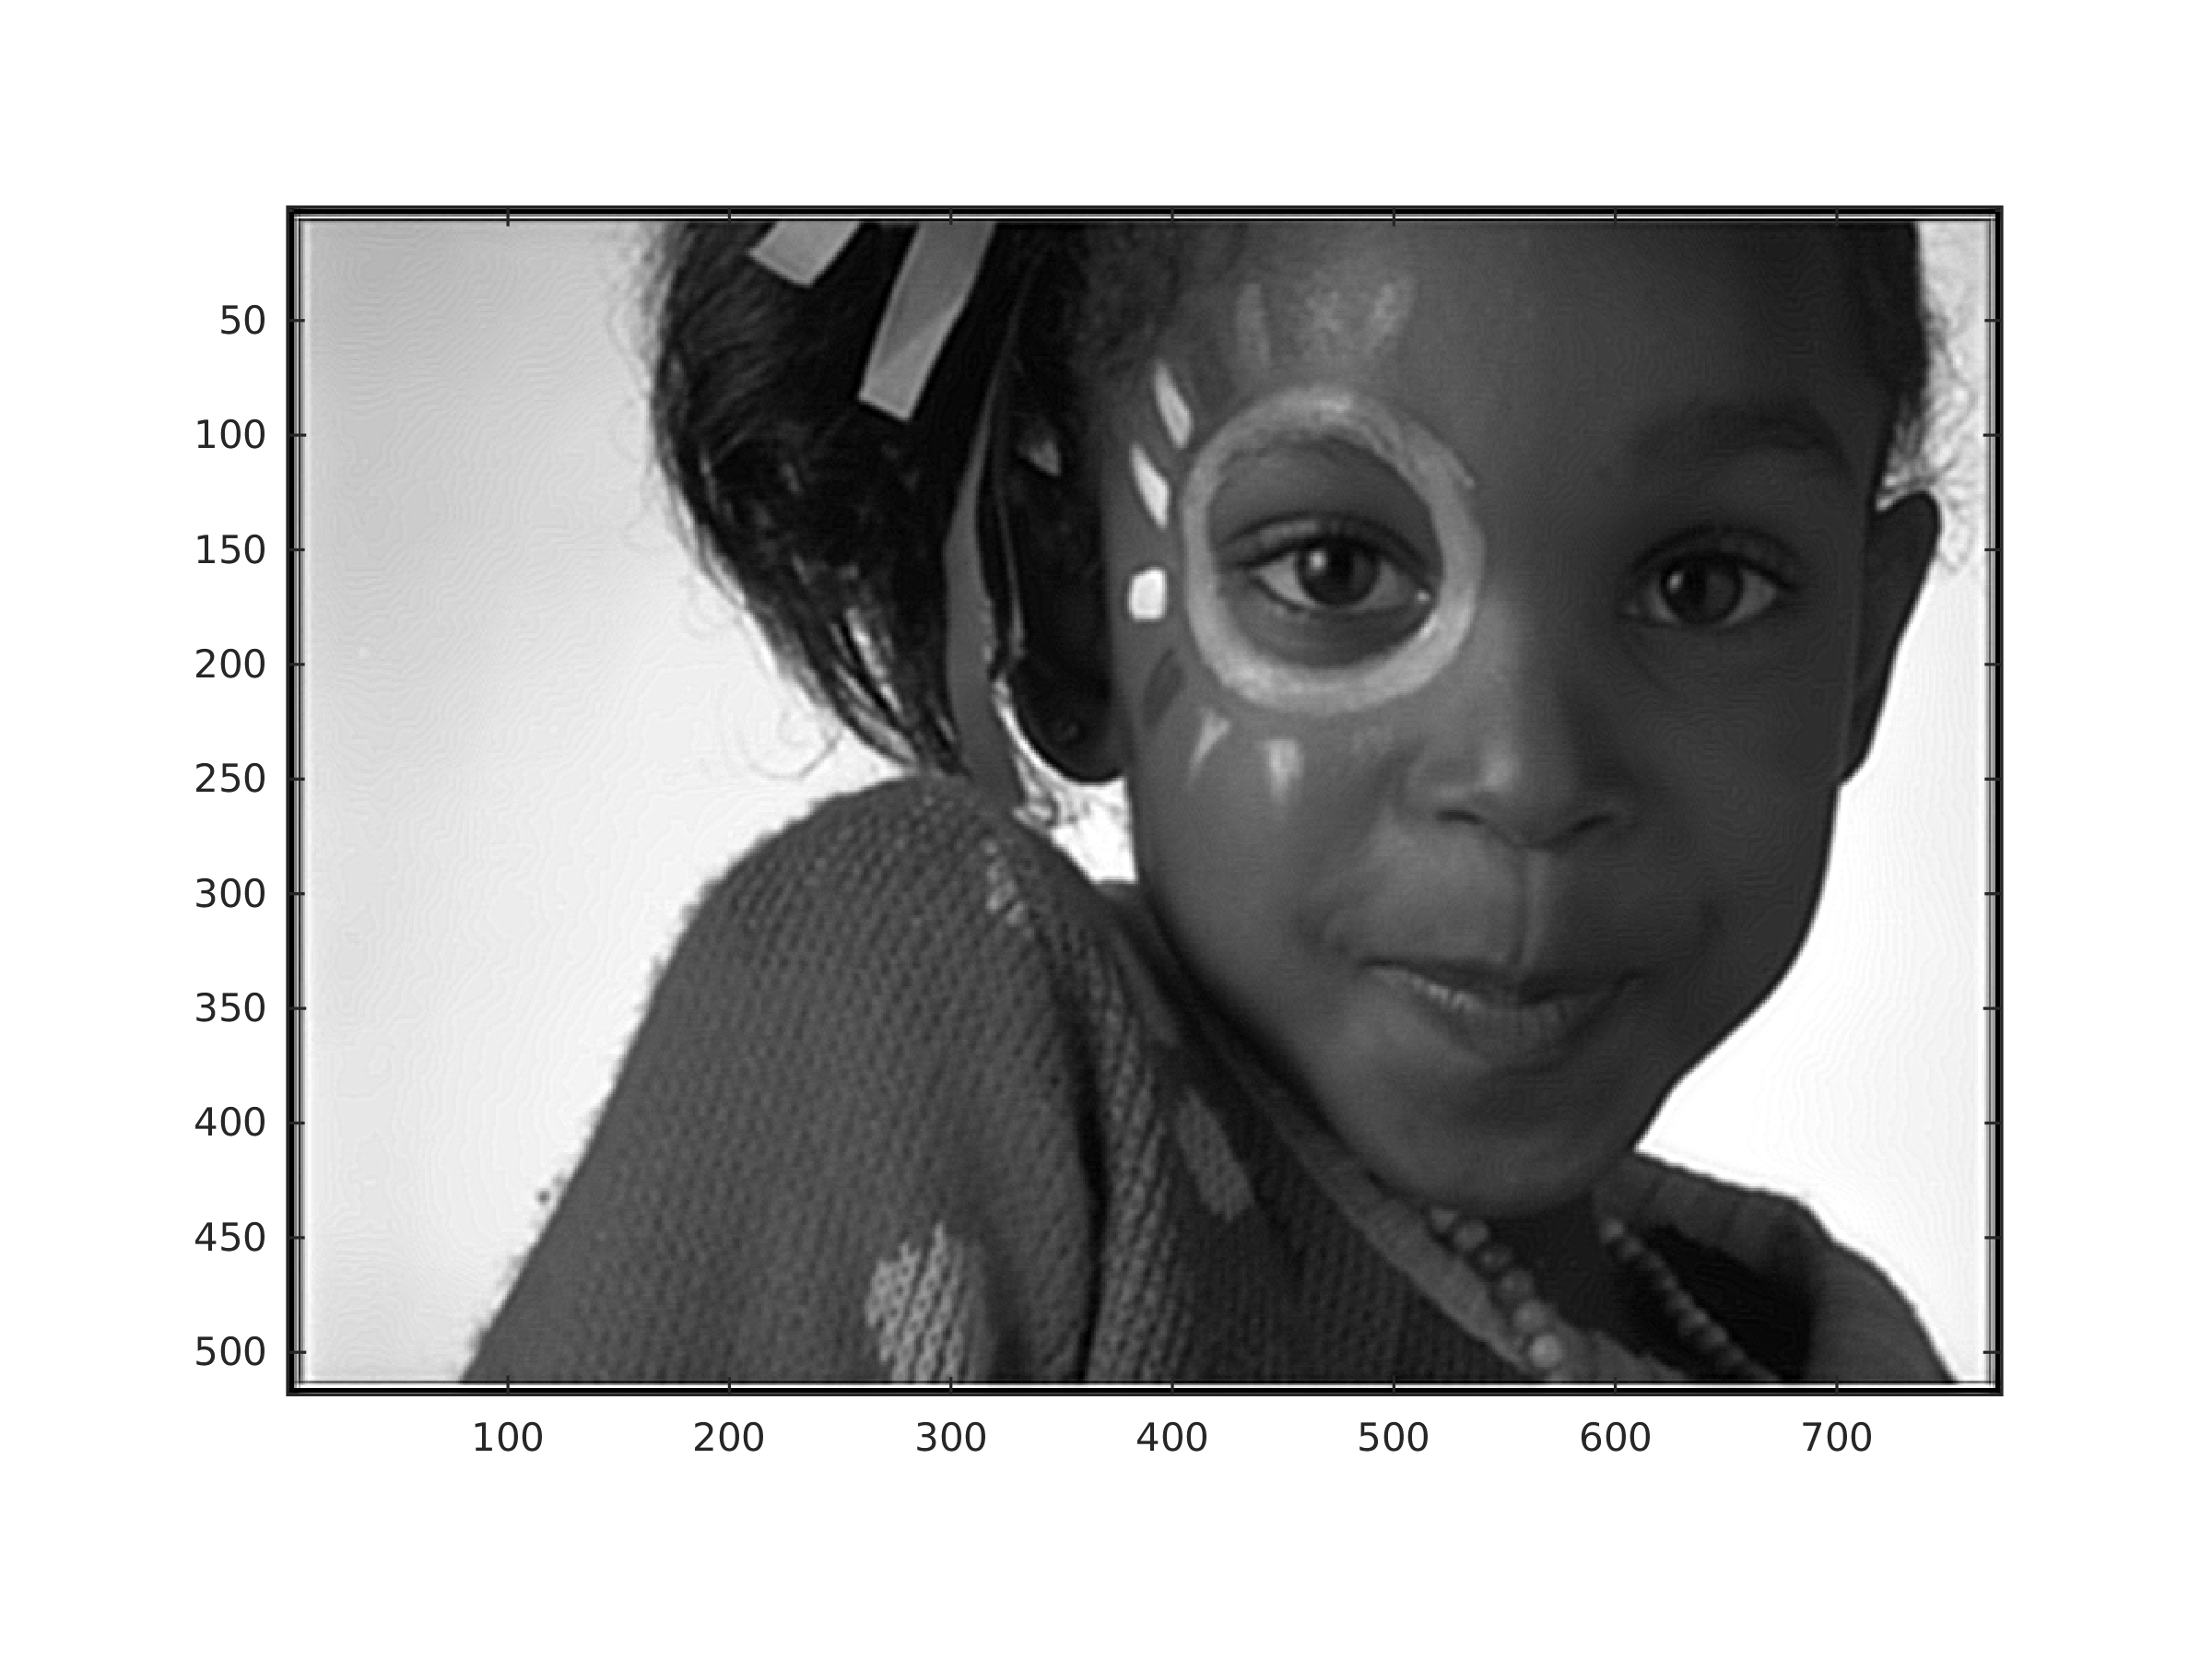
\includegraphics[width=1.0\textwidth]{nobl.png}
			\caption{Filtered Blurred Image}
		\end{subfigure}
		\begin{subfigure}{0.5\textwidth}
			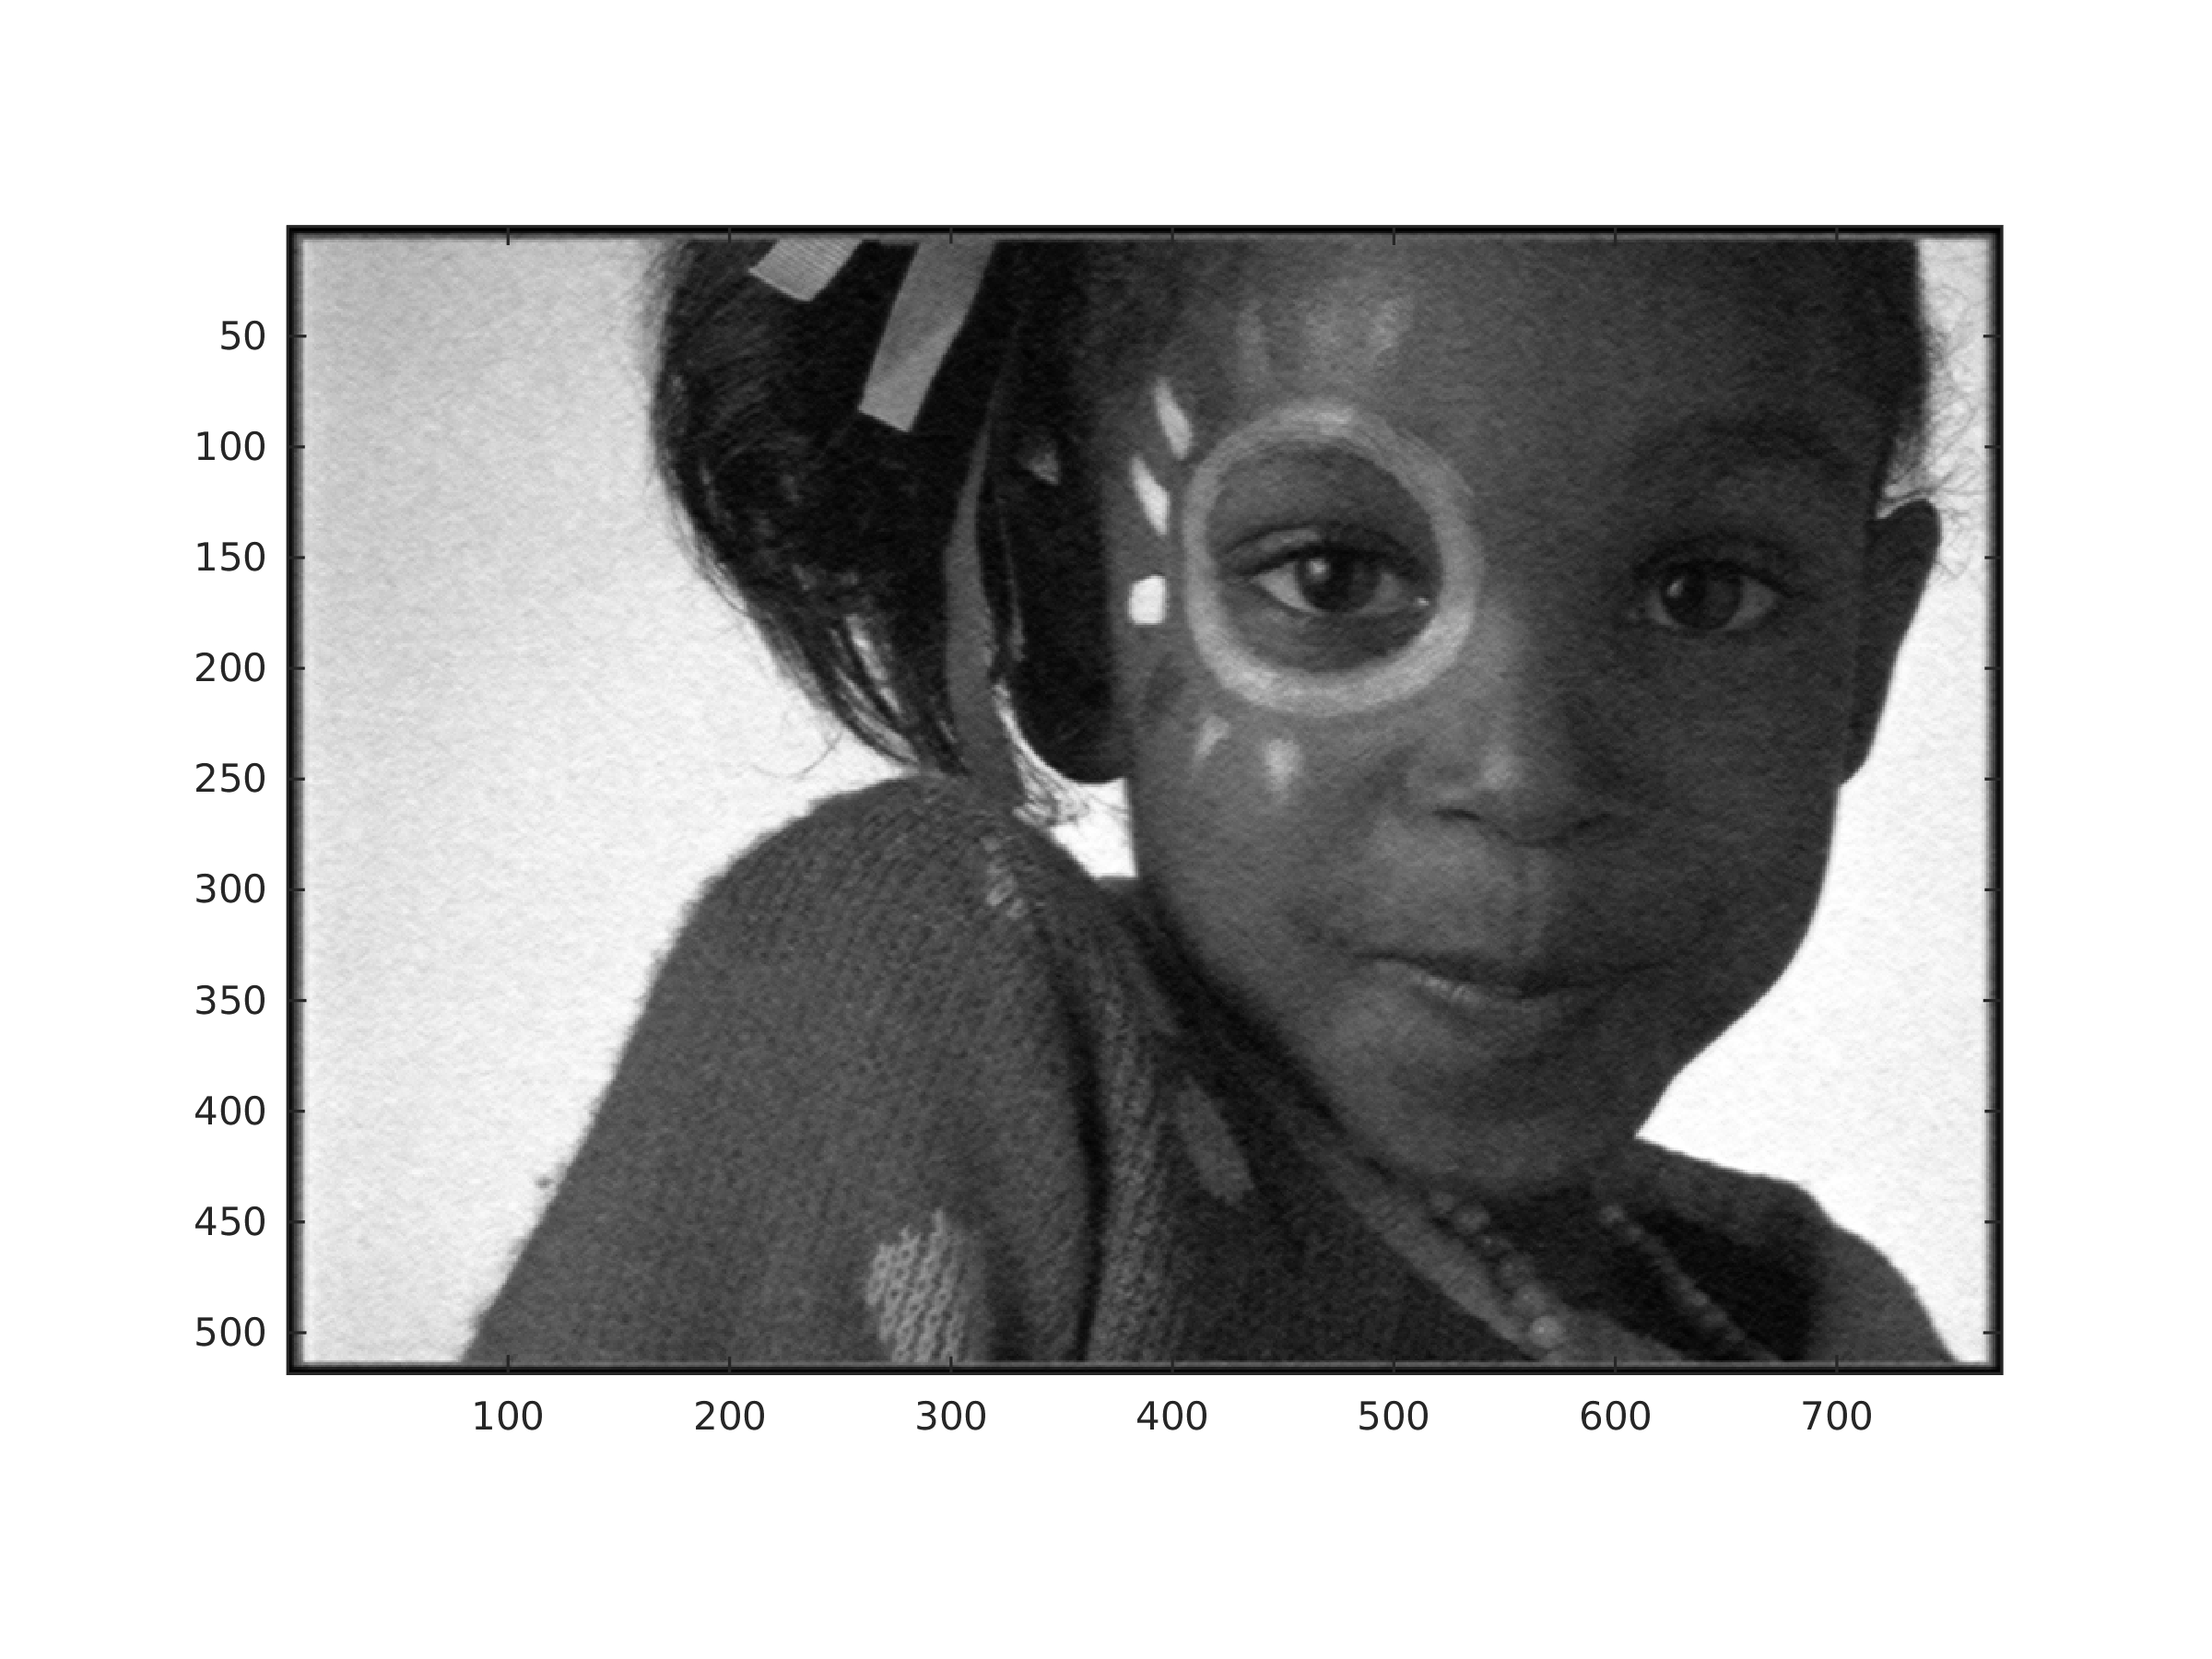
\includegraphics[width=1.0\textwidth]{non.png}
			\caption{Filtered Noisy Image}
		\end{subfigure}
		\begin{subfigure}{1.0\textwidth}
			\begin{center}
				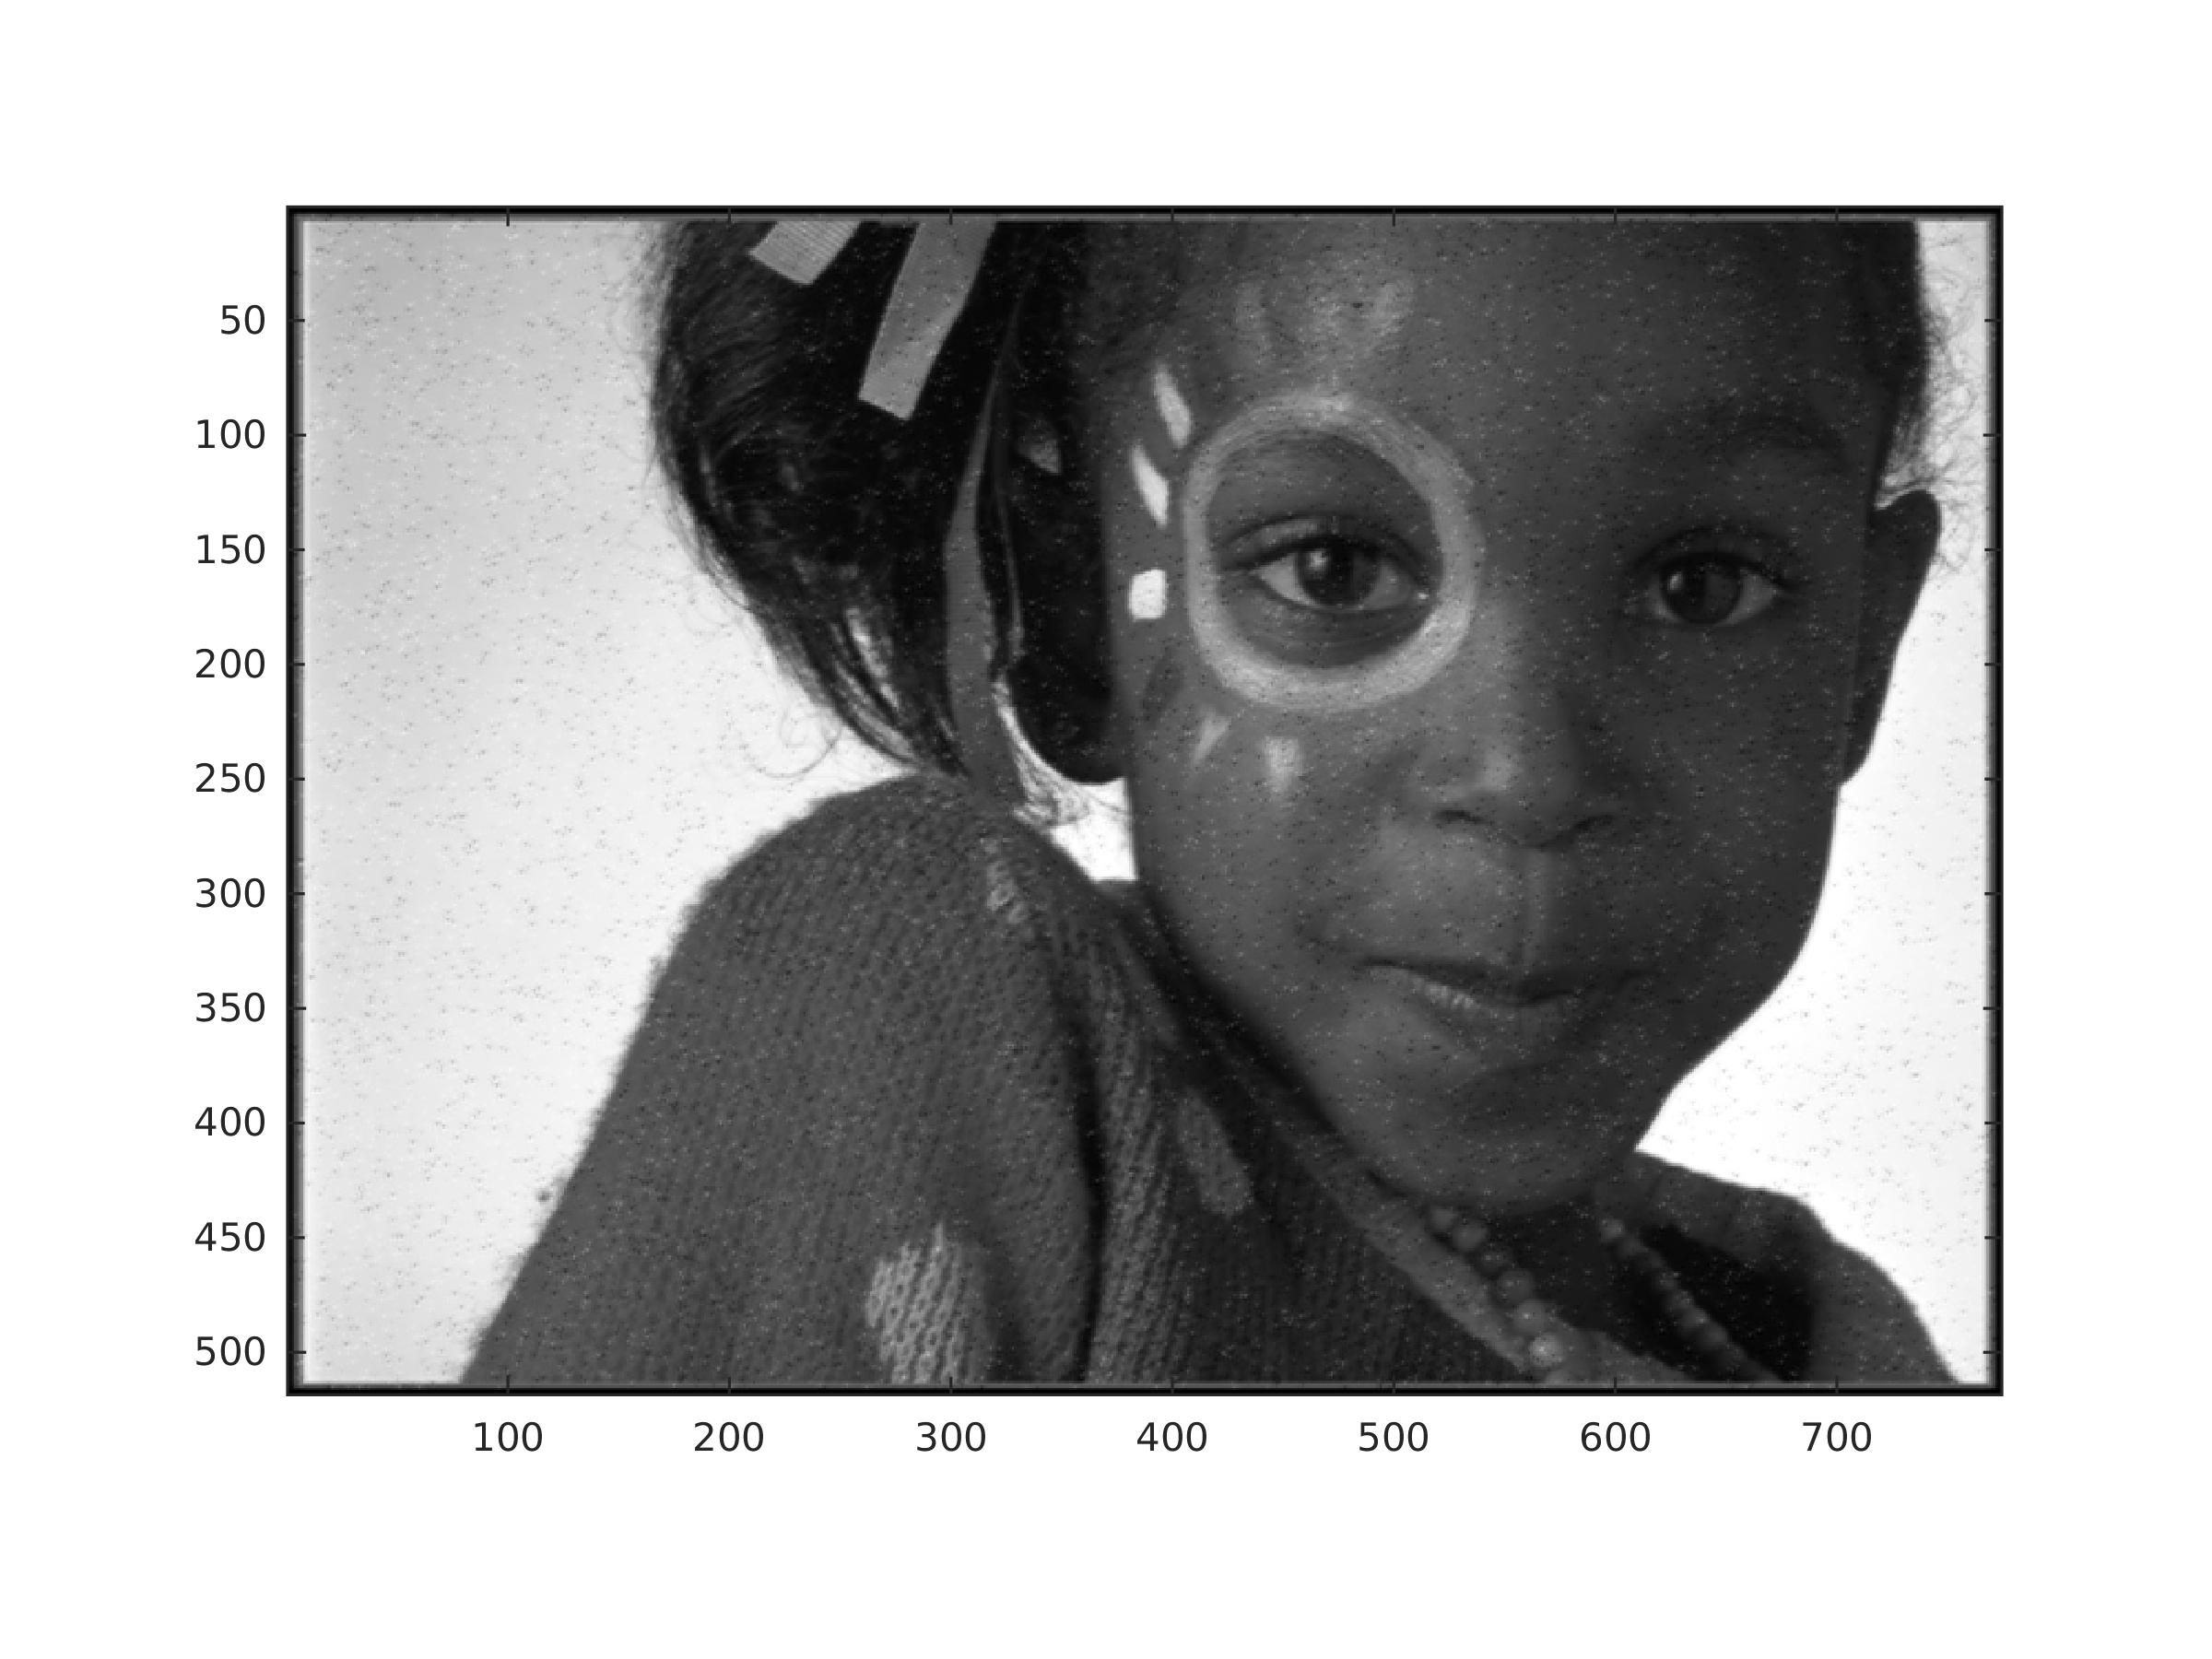
\includegraphics[width=0.5\textwidth]{nosp.png}
				\caption{Filtered Noisy Image with Spots}
			\end{center}
		\end{subfigure}
		\caption{Distorted Images After Optimal Filtering}	
	\end{figure}

\subsection{Results of MMSE Filters, $\theta^{\star}$}
	For the blurred image,
	\begin{align*}
		\theta^{\star} =
		\begin{bmatrix}
			1.7122 & 0.7401 & 0.9280 & 0.8153 & -0.9378 & -1.8137 & 1.8075 \\
		   -1.4864 & -1.8092 & -0.9006 & -0.5821& -2.9833 & 0.5828 & 1.3537 \\
		   -0.9434 & -2.7623 & 0.3063 & 2.9781 & 0.7147 & -2.7348 & -0.8187 \\
			2.0282 & -0.5532 & 3.6350 & 3.4485 & 3.2368 & -3.1583 & 0.6775 \\
			1.6263 & -3.0881 & -0.4136 & 5.0773 & -0.1598 & -1.4265 & 0.7996 \\
		   -0.3035 & −0.3035 & −0.3035 & −0.3035 & −0.3035 & −1.5040 & 0.9250 \\
			1.2638 & 1.2638 & 1.2382 & 1.8732 & −1.1491 & −1.2882 & 1.0076 \\
		\end{bmatrix}
	\end{align*}
	For the noisy image,
	\begin{align*}
		\theta^{\star} =
		\begin{bmatrix}
			0.0165 & -0.0055 & -0.0105 & -0.0091 & -0.0050 & -0.0044 & -0.0053 \\
			0.0259 &  0.0053 & -0.0125 & -0.0153 & -0.0222 &  0.0079 & -0.0043 \\
			0.0044 &  0.0355 &  0.0674 &  0.0476 &  0.0423 &  0.0307 &  0.0154 \\
			0.0050 &  0.0205 &  0.0731 &  0.2306 &  0.1117 &  0.0268 &  0.0127 \\
		   -0.0080 &  0.0464 &  0.0470 &  0.0891 &  0.0650 &  0.0088 &  0.0140 \\
			0.0302 &  0.0091 &  0.0290 & -0.0175 & -0.0118 & -0.0063 &  0.0183 \\
		   -0.0259 &  0.0066 & -0.0030 &  0.0011 &  0.0069 &  0.0192 &  0.0054 \\
		\end{bmatrix}
	\end{align*}
	For the noisy image with spots,
	\begin{align*}
		\theta^{\star} =
		\begin{bmatrix}
			0.0080 &  0.0017 & -0.0010 & -0.0014 &  0.0252 & -0.0099 & -0.0407 \\
			0.0048 & -0.0016 &  0.0042 & -0.0203 &  0.0023 & -0.0006 &  0.0162 \\
		   -0.0016 &  0.0558 &  0.0413 &  0.0350 &  0.0612 &  0.0313 & -0.0068 \\
		   -0.0050 &  0.0267 &  0.0968 &  0.2652 &  0.0965 &  0.0497 &  0.0100 \\
			0.0257 &  0.0435 &  0.0212 &  0.1492 &  0.0154 &  0.0143 &  0.0079 \\
		   -0.0209 &  0.0214 & -0.0196 & -0.0287 & -0.0412 &  0.0038 &  0.0129 \\
		   -0.0185 &  0.0196 &  0.0199 &  0.0083 &  0.0233 &  0.0131 & -0.0110 \\
		\end{bmatrix}
	\end{align*}
	
%----------------------------------------------------------------------------------------
%	SECTION 2
%----------------------------------------------------------------------------------------
\section{Weighted Median Filtering}

\subsection{Results of Median Filtering}
	\begin{figure}[h]
		\begin{subfigure}{0.5\textwidth}
			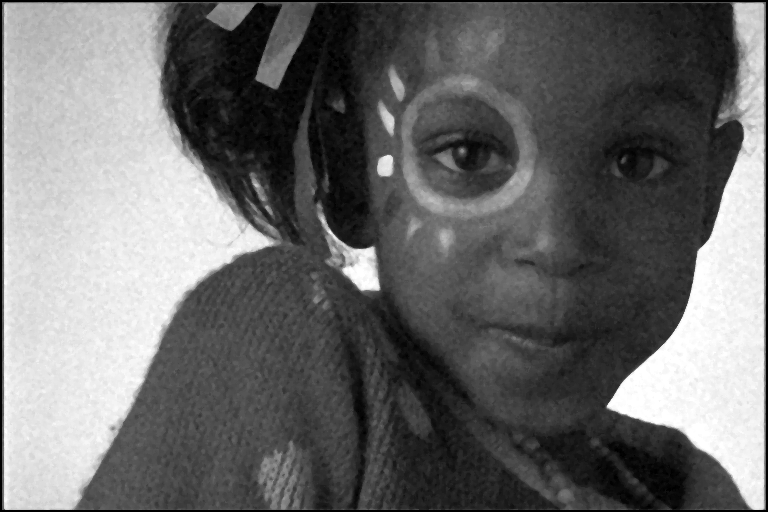
\includegraphics[width=1.0\textwidth]{cnon.png}
			\caption{Median Filtered Blurred Image}
		\end{subfigure}
		\begin{subfigure}{0.5\textwidth}
			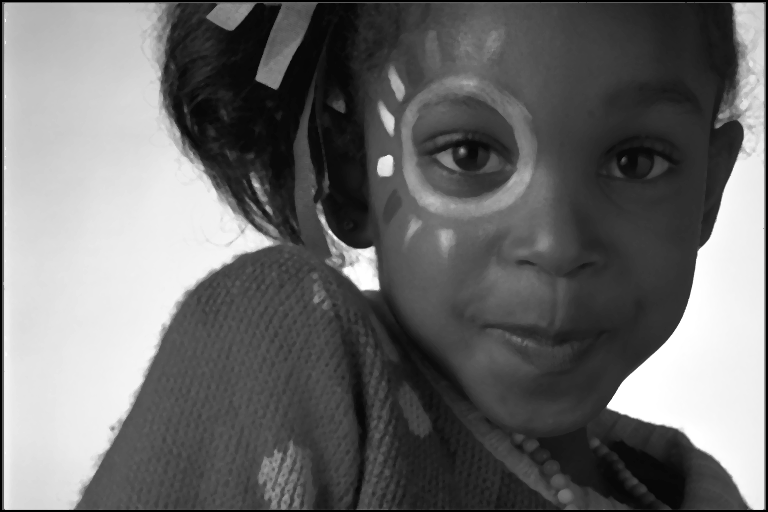
\includegraphics[width=1.0\textwidth]{cnsp.png}
			\caption{Median Filtered Noisy Image}
		\end{subfigure}
		\caption{Weighted Median Filtered Image}
	\end{figure}

\subsection{Code Listing}
	\subsubsection{medfilter.h}
		\inputminted[tabsize=4]{c}{medfilter.h}
	\subsubsection{medfilter.c}
		\inputminted[tabsize=4]{c}{medfilter.c}

\end{document}
